%\VignetteIndexEntry{MeSH.db}
\documentclass[11pt]{article}
\usepackage{Sweave}
\usepackage{amsmath}
\usepackage{hyperref}
\usepackage{cite}
\usepackage{Sweave}

\usepackage[numbers]{natbib}
\usepackage{amsmath}
\usepackage{amssymb}
\input{MeSH-concordance}
\usepackage{hyperref,url}
\usepackage[utf8]{inputenc}
\usepackage{comment}

\setlength{\textheight}{8.5in}
\setlength{\textwidth}{6in}
\setlength{\topmargin}{-0.25in}
\setlength{\oddsidemargin}{0.25in}
\setlength{\evensidemargin}{0.25in}
\newcommand{\Rpackage}[1]{{\textit{#1}}}

\usepackage{Sweave}
\begin{document}


\title{\bf How to use MeSH-related Packages}
\author{Koki Tsuyuzaki$^{1,4}$, Gota Morota$^2$, Takeru Nakazato$^3$ and Itoshi Nikaido$^4$.}
\maketitle
\begin{center}
\noindent
$^1$Department of Medical and Life Science, Tokyo University of Science.\\
\noindent
$^2$Department of Animal Science, University of Nebraska-Lincoln\\
\noindent
$^3$Database Center for Life Science, Research Organization of Information and Systems.\\
\noindent
$^4$Bioinformatics Research Unit, RIKEN Advanced Center for Computing and Communication.\\
\end{center}

\begin{center}
{\tt k.t.the-answer@hotmail.co.jp, dritoshi@gmail.com}
\end{center}
\tableofcontents

%%%%%%%%%%%%%%%%%%%%%%%%%%%%%%%%%%%%%%%%%%%%%%%%%%%%%%%%%%%%%%%%%%
%\clearpage
\newpage
\section{Introduction}
This document provides the way to use MeSH-related packages; \Rpackage{MeSH.db}, \Rpackage{MeSH.AOR.db}, \Rpackage{MeSH.PCR.db}, $MeSH.XXX.eg.db$-type packages, \Rpackage{MeSHDbi}, and \Rpackage{meshr} packages. MeSH (Medical Subject Headings) is the NLM (U. S. National Library of Medicine) controlled vocabulary used to manually index articles for MEDLINE/PubMed \cite{Nelson2004} and is a collection of a comprehensive life science vocabulary.
%%%%%%%%%%%%%%%%%%%%%%%%%%%%%%%%%%%%%%%%%%%%%%%%%%%%%%%%%%%%%%%%%%
\begin{figure}[ht]
\centering
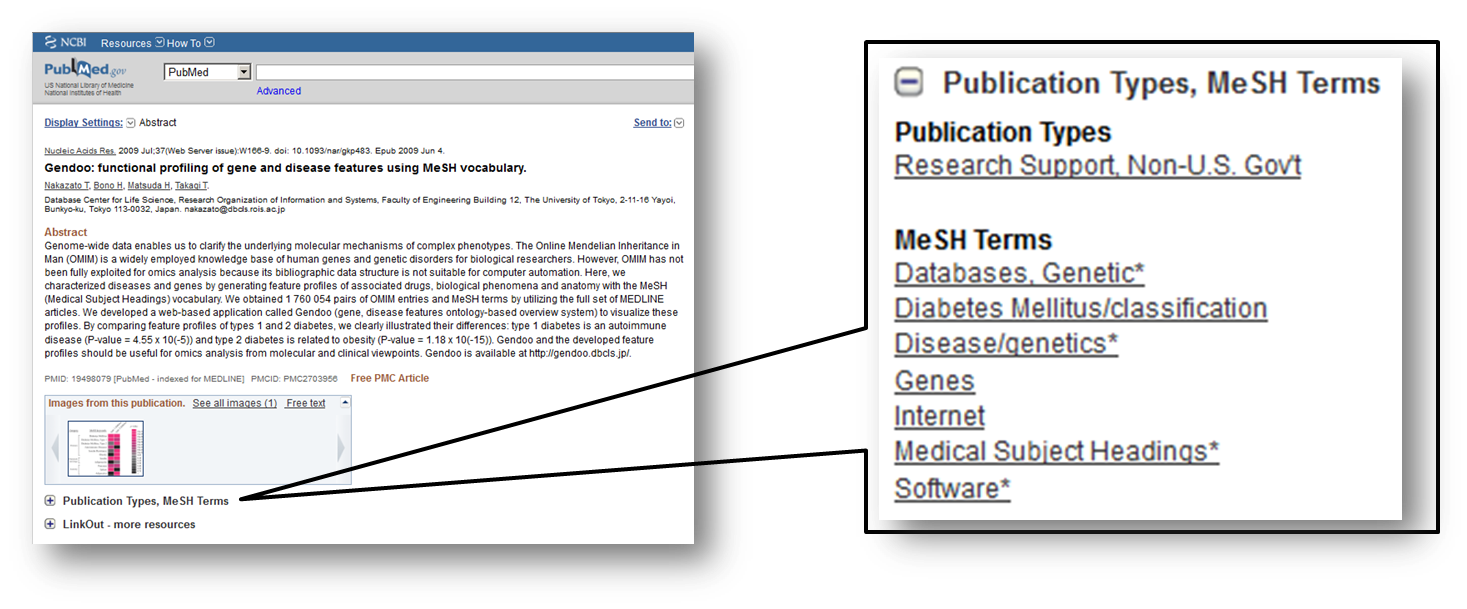
\includegraphics[width=\linewidth]{fig1.png}
\caption{MeSH Term}
\label{fig1}
\end{figure}
%%%%%%%%%%%%%%%%%%%%%%%%%%%%%%%%%%%%%%%%%%%%%%%%%%%%%%%%%%%%%%%%%%
MeSH contains more than 25,000 clinical and biological terms. The amount of MeSH term is about twice as large as that of GO (Gene Ontology)\cite{Ashburner2000} and its categories are also wider. MeSH in 2014 proposed its 19 categories and \Rpackage{MeSH.db} provides 16 of them, which are actually assigned to some MeSH terms. Each category is expressed as single capital alphabet as abbreviation defined by NLM. Therefore MeSH is an expected to be much detailed and exhaustive gene annotation tool. Some software or databases using MeSH are now proposed \cite{Nakazato2007, Nakazato2009, Saurin2010, Sartor2012}.
%%%%%%%%%%%%%%%%%%%%%%%%%%%%%%%%%%%%%%%%%%%%%%%%%%%%%%%%%%%%%%%%%%
\begin{center}
  \begin{table}[htbp]
    \begin{tabular}{|c|l|}\hline
      Abbreviation & Category \\ \hline \hline
      A & Anatomy \\ \hline
      B & Organisms \\ \hline
      C & Diseases \\ \hline
      D & Chemicals and Drugs \\ \hline
      E & Analytical, Diagnostic and Therapeutic Techniques and Equipment \\ \hline
      F & Psychiatry and Psychology \\ \hline
      G & Phenomena and Processes \\ \hline
      H & Disciplines and Occupations \\ \hline
      I & Anthropology, Education, Sociology and Social Phenomena \\ \hline
      J & Technology and Food and Beverages \\ \hline
      K & Humanities \\ \hline
      L & Information Science \\ \hline
      M & Persons \\ \hline
      N & Health Care \\ \hline
      V & Publication Type \\ \hline
      Z & Geographical Locations \\ \hline
\end{tabular}
  \end{table}
\end{center}
%%%%%%%%%%%%%%%%%%%%%%%%%%%%%%%%%%%%%%%%%%%%%%%%%%%%%%%%%%%%%%%%%%
This vignette introduces R/Bioconductor packages for handling MeSH in R. Original MeSH data is accessible by NLM FTP site (\url{http://www.nlm.nih.gov/mesh/filelist.html}). The data are downloadable as plain-text format (ASCII MeSH; d2015.bin / q2015.bin). These files were pre-processed by our data-processing pipeline (figure 2) and corresponding information is summarized as a table in SQLite3 file and packed into \Rpackage{MeSH.db}, \Rpackage{MeSH.AOR.db}, and \Rpackage{MeSH.PCR.db}.

\clearpage
\subsection{About MeSH}
\Rpackage{MeSH.db} provides the corresponding table which contains MeSH ID, MeSH term, MeSH category, synonym, qualifier ID, and qualifier term. Qualifier term means more rough annotation (subheadings) than MeSH. MeSH has hierarchical structure like GO. Such structure is provided as \Rpackage{MeSH.AOR.db} (AOR: ancestor-offspring Relationships) and \Rpackage{MeSH.PCR.db} (PCR: parent-child Relationships as corresponding table.
%%%%%%%%%%%%%%%%%%%%%%%%%%%%%%%%%%%%%%%%%%%%%%%%%%%%%%%%%%%%%%%%%%
\begin{figure}[ht]
\centering
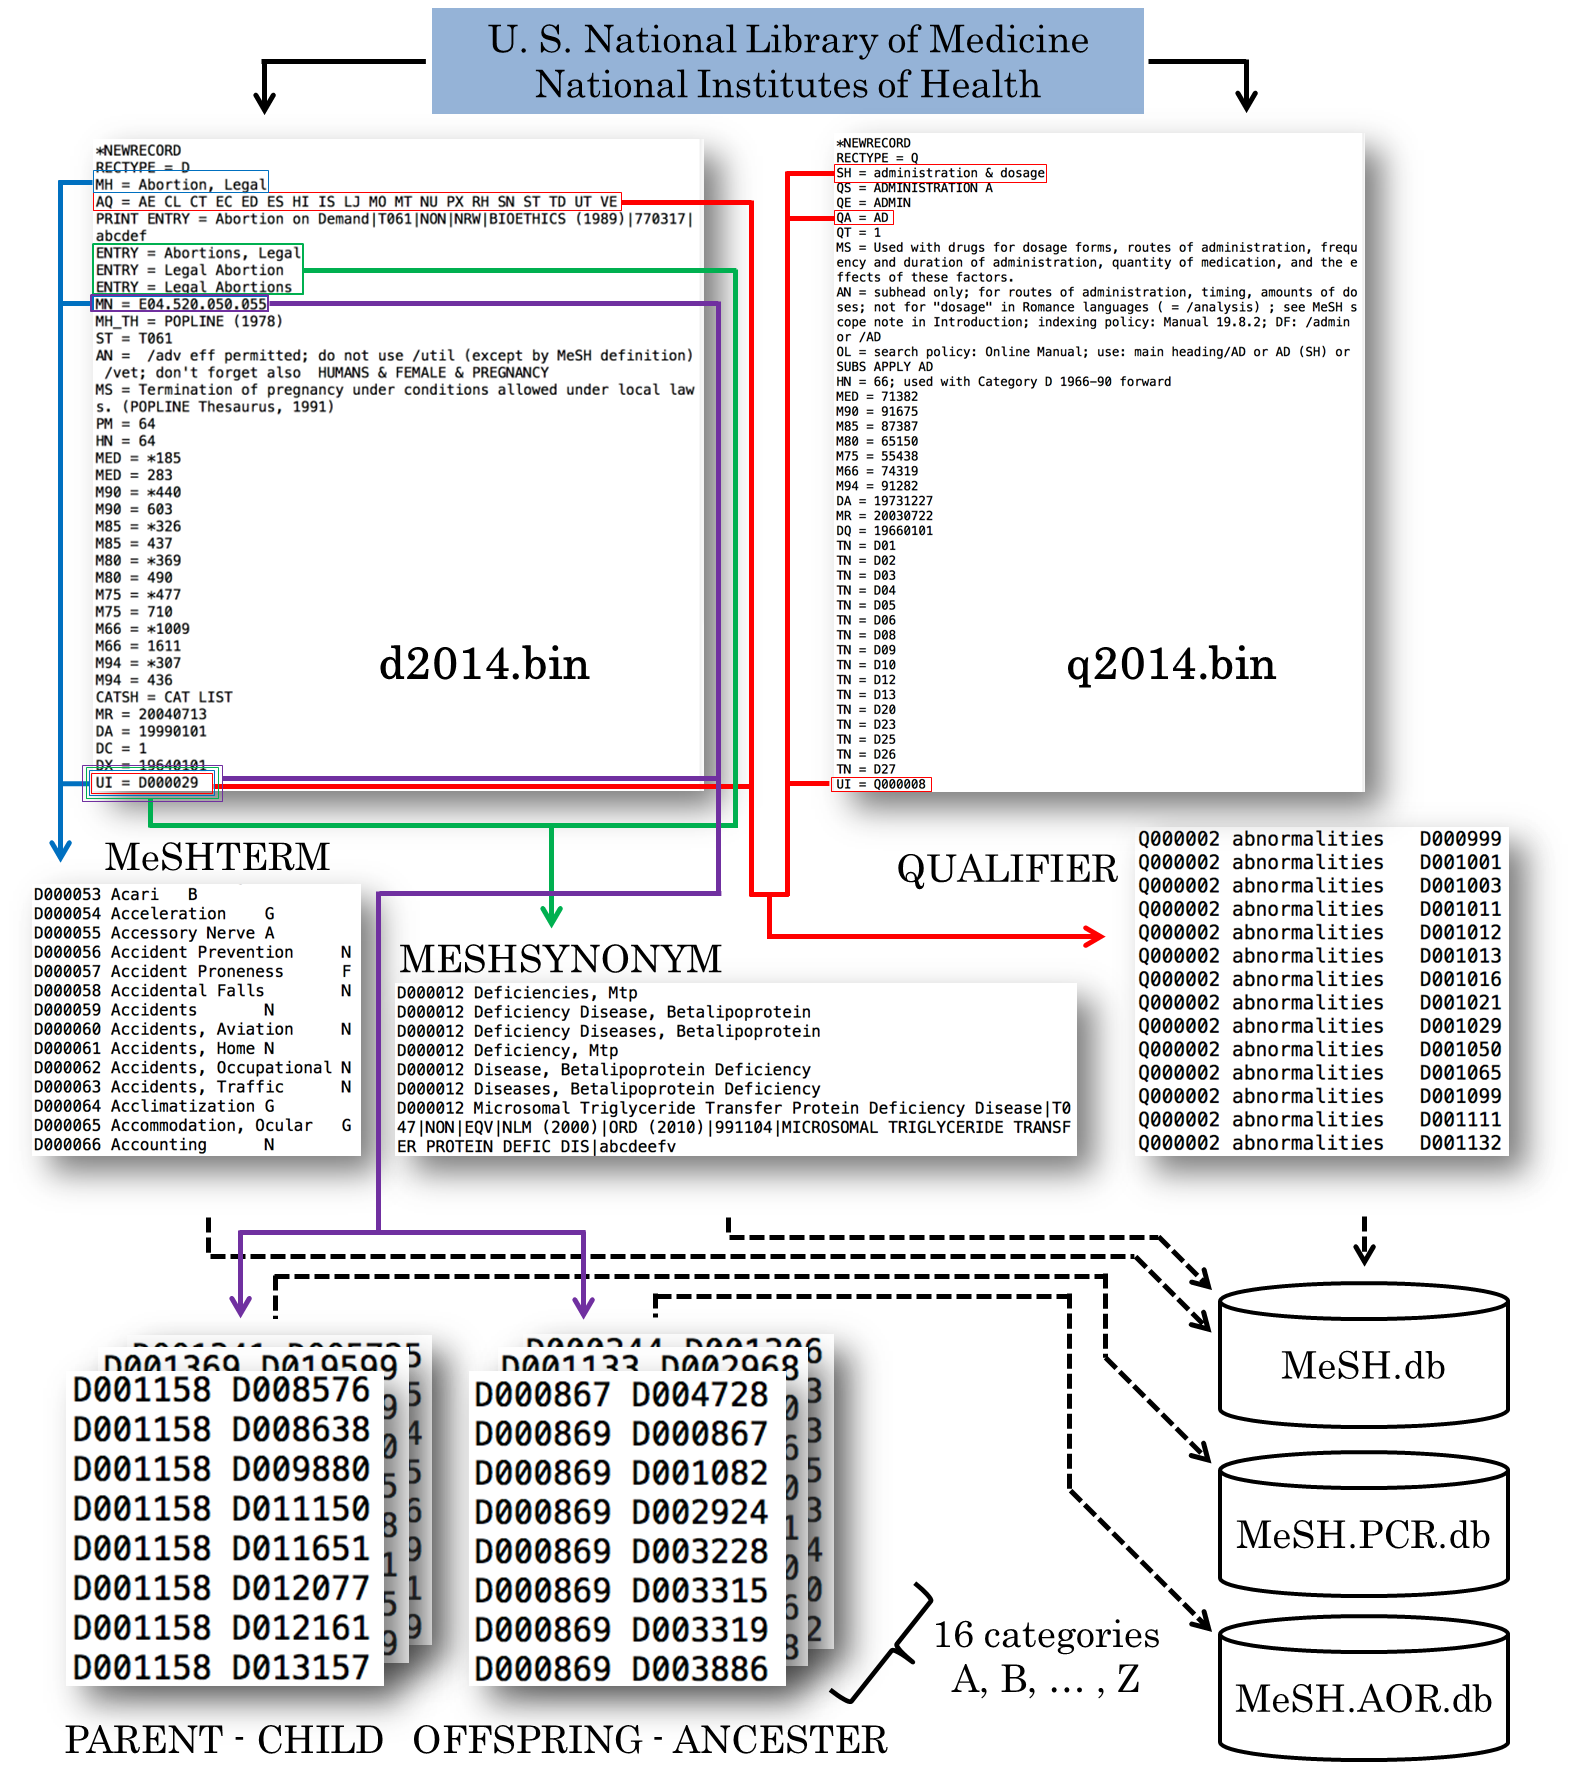
\includegraphics[width=14.0cm]{fig2.png}
\caption{Data pre-process for MeSH.db}
\label{fig2}
\end{figure}
%%%%%%%%%%%%%%%%%%%%%%%%%%%%%%%%%%%%%%%%%%%%%%%%%%%%%%%%%%%%%%%%%%
\clearpage
\subsection{The correspondence between MeSH ID and NCBI Entrez Gene ID}
MeSH.XXX.eg.db (XXX is an abbreviation of species name such as Hsa: Homo sapiens) packages provide the correspondence between Entrez Gene IDs and NLM MeSH IDs. Such correspondence in wide variety of organisms are summarized as each MeSH.XXX.eg.db by three way of methods, Gendoo\cite{Nakazato2009}, gene2pubmed, and RBBH (reciprocal BLAST best Hit).

Gendoo is the web-application based on text-mining of PubMed. Co-occurrence relations in PubMed document are exhaustively retrieved and much relevant correspondence are filtered by some information science techniques.

gene2pubmed is the correspondence between Entrez Gene IDs and NLM PubMed IDs. These relationship is manually assigned by NCBI curator teams. We also summarized the relationship between MeSH Terms and PubMed IDs from licensed-PubMed, then merged as Gene IDs - MeSH IDs correspondence.

For some minor species including non-model organisms, which have no sufficient databases for annotation, we defined 15 well-annotated organisms and 100 minor-organisms, then conducted RBBH between all possible combinations using BLASTP search.
%%%%%%%%%%%%%%%%%%%%%%%%%%%%%%%%%%%%%%%%%%%%%%%%%%%%%%%%%%%%%%%%%%
\begin{center}
  \begin{table}[htbp]
    \begin{tabular}{|c|l|}\hline
      Method & Way of corresponding Entrez Gene IDs and MeSH IDs \\ \hline \hline
      Gendoo & Text-mining \\ \hline
      gene2pubmed & Manual curation by NCBI teams \\ \hline
      RBBH & sequence homology with BLASTP search (E-value < $10^{-50}$) \\ \hline
\end{tabular}
  \end{table}
\end{center}
%%%%%%%%%%%%%%%%%%%%%%%%%%%%%%%%%%%%%%%%%%%%%%%%%%%%%%%%%%%%%%%%%%

%%%%%%%%%%%%%%%%%%%%%%%%%%%%%%%%%%%%%%%%%%%%%%%%%%%%%%%%%%%%%%%%%%
\begin{figure}[ht]
\centering
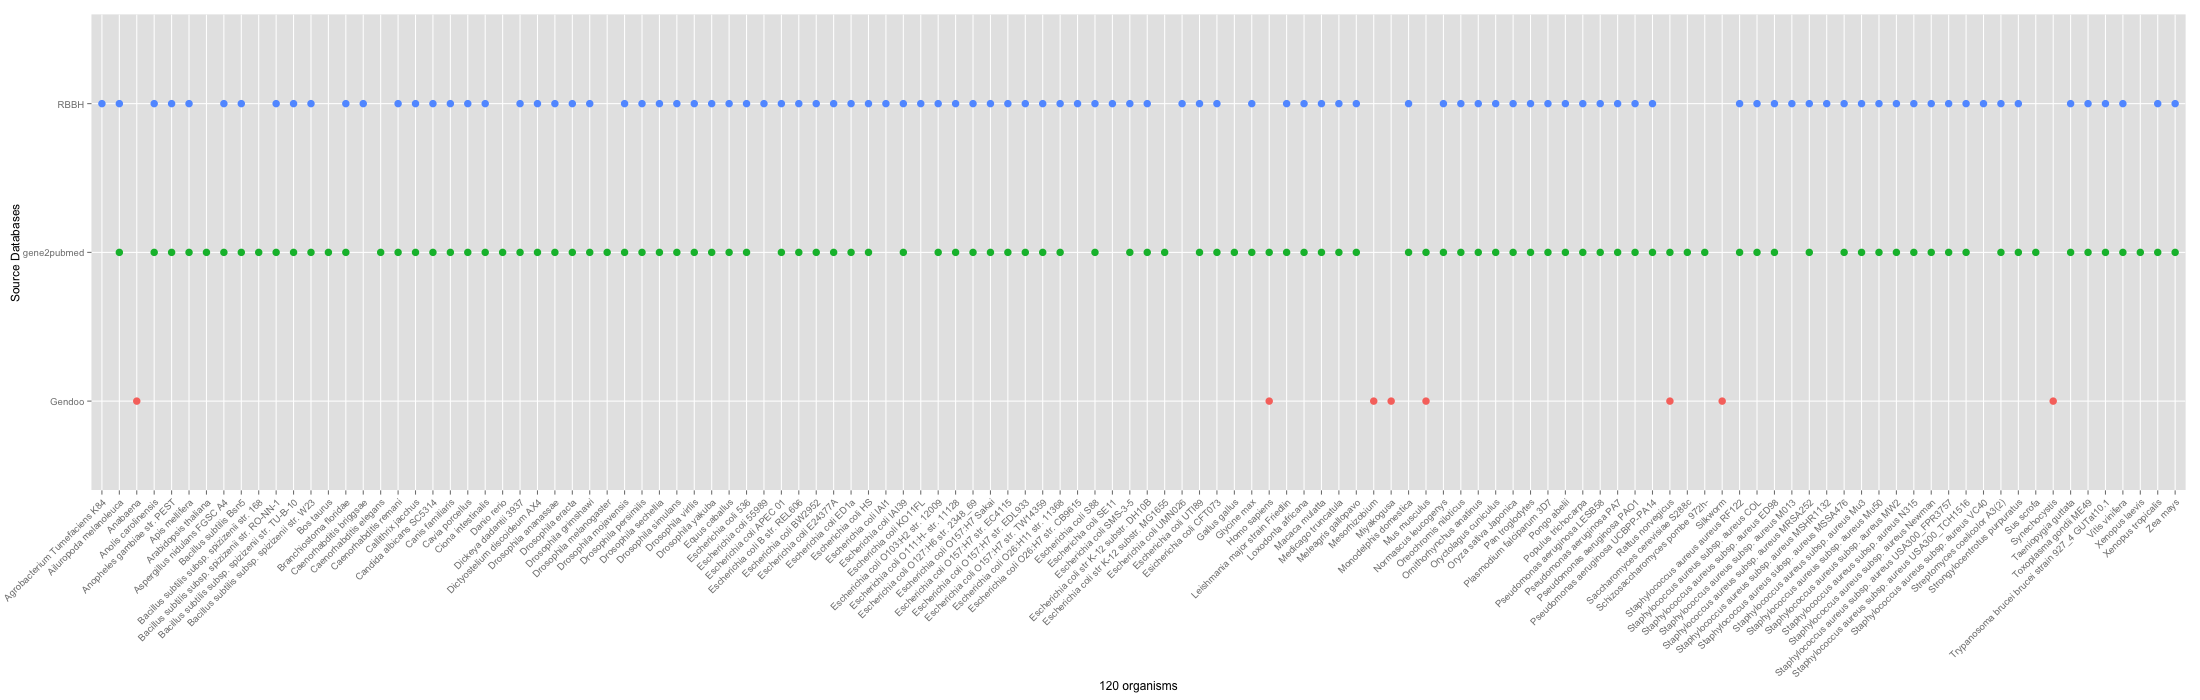
\includegraphics[width=\linewidth,angle=270]{fig3.png}
\caption{120 organisms for MeSH.XXX.eg.db and those source databases}
\label{fig3}
\end{figure}
%%%%%%%%%%%%%%%%%%%%%%%%%%%%%%%%%%%%%%%%%%%%%%%%%%%%%%%%%%%%%%%%%%
\clearpage
\subsection{Database interface package for MeSH-related packages}
We also implemented a database interface (DBI) package named \Rpackage{MeSHDbi}. This package is important because of two reasons. First reason is a unification of DBI functions for MeSH-related packages. \Rpackage{MeSH.db}, \Rpackage{MeSH.AOR.db}, \Rpackage{MeSH.PCR.db}, and $MeSH.XXX.eg.db$ packages inherit the MeSHDb-class defined by \Rpackage{MeSHDbi} and behavior of these packages is uniformly designed. Second reason is supporting construction of user's original MeSH.XXX.eg.db package. Due to the rapid development of DNA sequence technology, wide variety of genome sequences are more and more determined and the correspondence of Gene IDs and MeSH IDs may be designed by many databases \cite{Nakazato2007, Nakazato2009, Saurin2010, Sartor2012}. Therefore, we prepared the function to create MeSH.XXX.eg.db package for a situation in which users can retrieved the relationship between Gene IDs and MeSH IDs by some means.

\subsection{MeSH term enrichment analysis}
To analyze MeSH-related packages with omics data, we implement \Rpackage{meshr} package, which is for conducting enrichment analysis using MeSH data. This package internally imports \Rpackage{MeSH.db}, \Rpackage{MeSH.AOR.db}, \Rpackage{MeSH.PCR.db} and $MeSH.XXX.eg.db$, then conducts enrichment analysis to detect highlly enriched MeSH terms in gene sets of interesting species.
%%%%%%%%%%%%%%%%%%%%%%%%%%%%%%%%%%%%%%%%%%%%%%%%%%%%%%%%%%%%%%%%%%
\begin{figure}[ht]
\centering
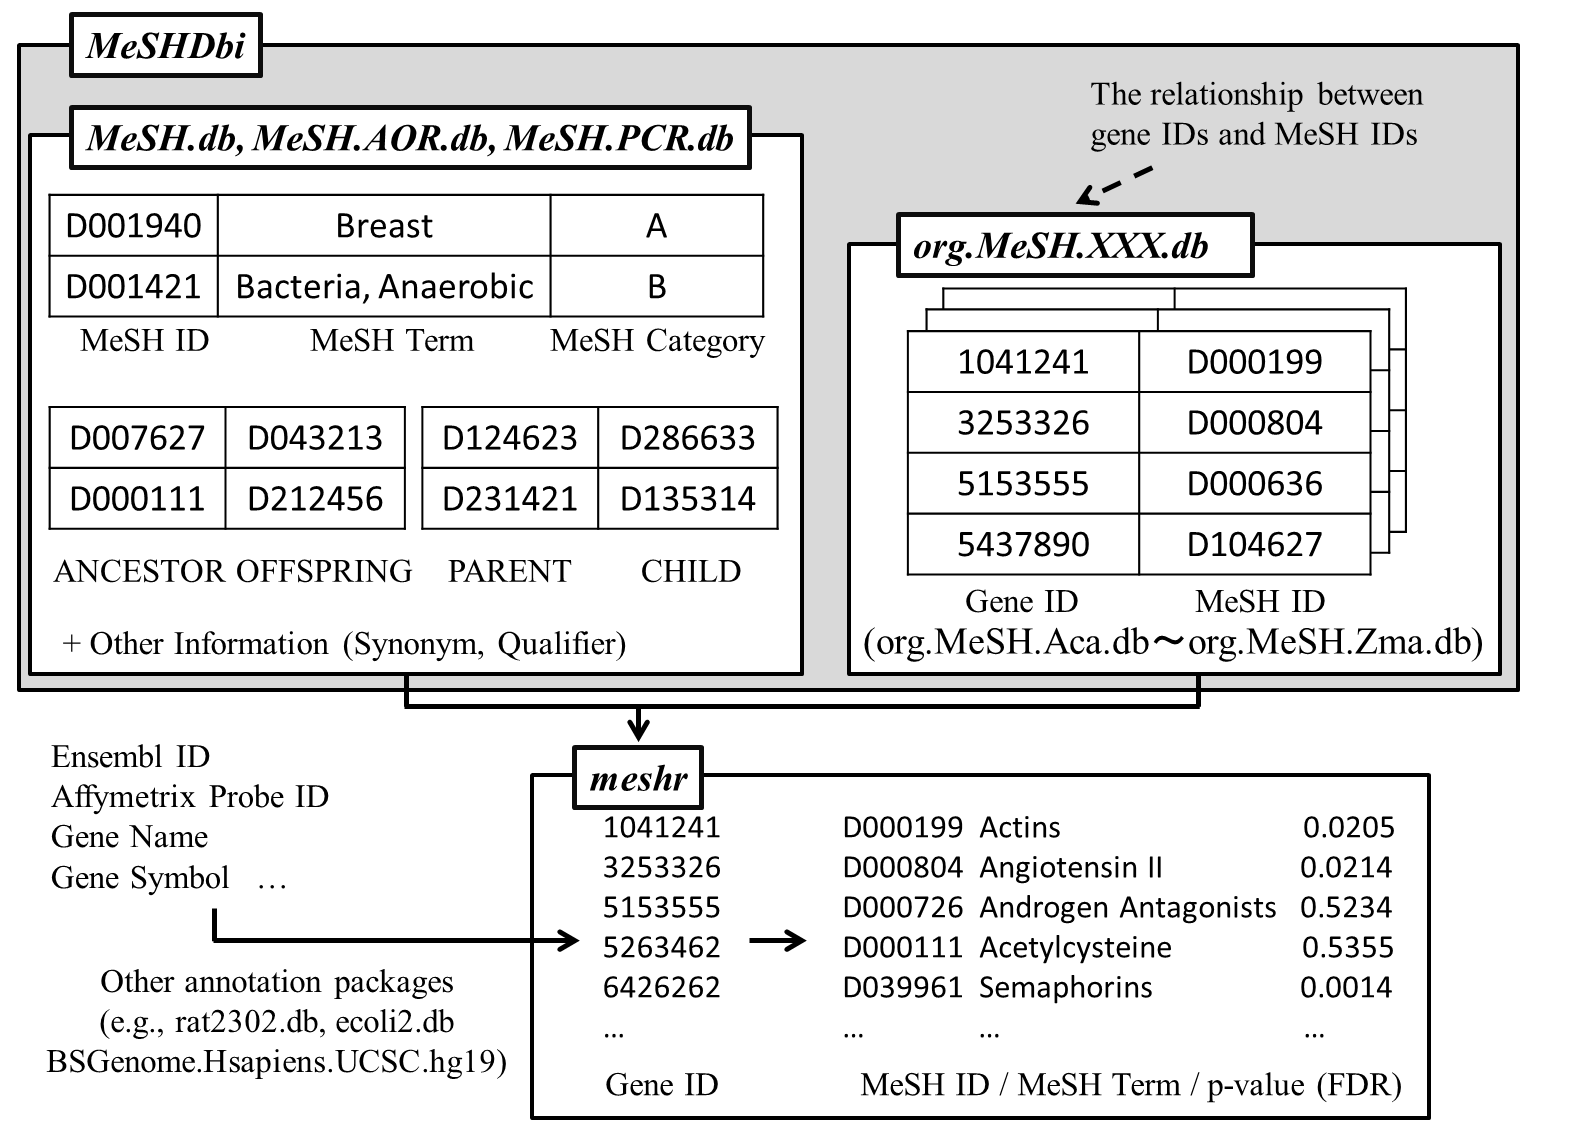
\includegraphics[width=\linewidth]{fig4.png}
\caption{The relationship of meshr and other MeSH-related packages}
\label{fig4}
\end{figure}
%%%%%%%%%%%%%%%%%%%%%%%%%%%%%%%%%%%%%%%%%%%%%%%%%%%%%%%%%%%%%%%%%%
\clearpage
\section{Exercise}
\subsection{Access MeSH Term}
\subsubsection{columns, keytypes, keys, and select}
In our packages, all data are extracted by only 4 functions defined by \Rpackage{AnnotationDbi}; $\bf{keytypes}$, $\bf{columns}$, $\bf{keys}$ and $\bf{select}$. In this section, we demonstrate how to use these functions by using \Rpackage{MeSH.db}.

At first, install and load the \Rpackage{MeSH.db}.
\begin{center}
\begin{Schunk}
\begin{Sinput}
> library(MeSH.db)
\end{Sinput}
\end{Schunk}
\end{center}

ls function shows all objects in this package. MeSH.db object is generated. This is also package's name and all MeSH-related packages provide the object named as package name (e.g., $MeSH.db$, $MeSH.Mmu.eg.db$).
\begin{center}
\begin{Schunk}
\begin{Sinput}
> ls("package:MeSH.db")
> MeSH.db
\end{Sinput}
\end{Schunk}
\end{center}

Here, we use $\bf{columns}$, $\bf{keytypes}$, $\bf{keys}$ and $\bf{select}$ against MeSH.db.\\

$\bf{columns}$ returns the rows which we can retrieve in MeSH.db.
\begin{center}
\begin{Schunk}
\begin{Sinput}
> columns(MeSH.db)
\end{Sinput}
\end{Schunk}
\end{center}

$\bf{keytypes}$ returns the rows which can be used as the optional parameter in $\bf{keys}$ and $\bf{select}$ functions against MeSH.db.

\begin{center}
\begin{Schunk}
\begin{Sinput}
> keytypes(MeSH.db)
\end{Sinput}
\end{Schunk}
\end{center}

\newpage
$\bf{keys}$ function returns the value of keytype.
\begin{center}
\begin{Schunk}
\begin{Sinput}
> k <- keys(MeSH.db, keytype = "MESHID")
> length(k)
> head(k)
\end{Sinput}
\end{Schunk}
\end{center}

$\bf{select}$ function returns rows in particular columns, which are having user-specified keys. This function provides the data as a dataframe. Now, we will retrieve the rows in which MESHID is equivalent to MESHTERM.
\begin{center}
\begin{Schunk}
\begin{Sinput}
> select(MeSH.db, keys = k[1:10], columns = c("MESHID", "MESHTERM"), 
+     keytype = "MESHID")
\end{Sinput}
\end{Schunk}
\end{center}

%\clearpage
\newpage
\subsubsection{Annotation of $Leukemia$}
Next, we will retrieve some information about $Leukemia$ by our packages.

$\bf{select}$ function retrieves rows in which MESHTERM is "$Leukemia$" in the MeSH.db table.
\begin{center}
\begin{Schunk}
\begin{Sinput}
> LEU <- select(MeSH.db, keys = "Leukemia", columns = c("MESHID", 
+     "MESHTERM", "CATEGORY", "SYNONYM"), keytype = "MESHTERM")
> LEU
\end{Sinput}
\end{Schunk}
\end{center}

$\bf{select}$ function shows that MESHID of $Leukemia$ is D007938 and $Leukemia$ is categorized as C (Diseases). $Leukemia$ has some synonyms like $Leucocythaemias$, $Leucocythaemia$, $Leucocythemias$ and $Leukemias$.

As mentioned above, MeSH has hierarchical structures. \Rpackage{MeSH.AOR.db} and \Rpackage{MeSH.PCR.db} packages provide such hierarchical information of MeSH. For example, \Rpackage{MeSH.AOR.db} enable us to examine the top terms of $Leukemia$.

\begin{center}
\begin{Schunk}
\begin{Sinput}
> library("MeSH.AOR.db")
> ANC <- select(MeSH.AOR.db, keys = "D007938", columns = c("ANCESTOR", 
+     "OFFSPRING"), keytype = "OFFSPRING")
> ANC
\end{Sinput}
\end{Schunk}
\end{center}
D009370 has found above $Leukemia$.\\

These MeSH IDs can be translated to MeSH Term.
\begin{center}
\begin{Schunk}
\begin{Sinput}
> select(MeSH.db, keys = ANC[1, 1], columns = c("MESHTERM"), keytype = "MESHID")
\end{Sinput}
\end{Schunk}
\end{center}
In this way, we can specify that $Leukemia$ is categorized as one of $Neoplasms by Histologic Type$.

Once keytype-parameter set to opposite direction (OFFSPRING to ANCESTOR), other MeSH IDs in lower hierarchies also can be retrieved.
\begin{center}
\begin{Schunk}
\begin{Sinput}
> OFF <- select(MeSH.AOR.db, keys = "D007938", columns = c("ANCESTOR", 
+     "OFFSPRING"), keytype = "ANCESTOR")
> OFF
> select(MeSH.db, keys = OFF[, 2], columns = c("MESHTERM"), keytype = "MESHID")
\end{Sinput}
\end{Schunk}
\end{center}
There are a lot of MeSH terms, which means $Leukemia$ has many lower hierarchies.\\

\Rpackage{MeSH.PCR.db} provides the directly lower (or upper) terms.
\begin{center}
\begin{Schunk}
\begin{Sinput}
> library("MeSH.PCR.db")
> CHI <- select(MeSH.PCR.db, keys = LEU[1, 1], columns = c("PARENT", 
+     "CHILD"), keytype = "PARENT")
> head(CHI)
> head(select(MeSH.db, keys = CHI[, 2], columns = c("MESHTERM"), 
+     keytype = "MESHID"))
\end{Sinput}
\end{Schunk}
\end{center}

$Leukemia$ has a lot of subtypes like $Avian Leukosis$, $Blast Crisis$, $Leukemia, Erythroblastic, Acute$ and so on.

%%%%%%%%%%%%%%%%%%%%%%%%%%%%%%%%%%%%%%%%%%%%%%%%%%%%%%%%%%%%%%%%%
\clearpage
\subsubsection{Other functions}
Some optional functions for much complex data acquisition are also provided. In this section, users may need some basic $SQL$ knowledge (see also \Rpackage{RSQLite}).

$dbInfo$ returns the information of the package. $dbfile$ returns the directory where sqlite file is stored. $dbschema$ returns the schema of database. $dbconn$ returns the connection constructed by \Rpackage{RSQLite}.
\begin{center}
\begin{Schunk}
\begin{Sinput}
> dbInfo(MeSH.db)
> dbfile(MeSH.db)
> dbschema(MeSH.db)
> dbconn(MeSH.db)
\end{Sinput}
\end{Schunk}
\end{center}

$dbschema$ shows the data is stored as a table named "DATA" in the sqlite database and the table has six columns; MESHID, MESHTERM, CATEGORY, SYNONYM, QUALIFIERID, and QUALIFIER. Therefore, we can retrieve data by much complex SQL query like below;
\begin{center}
\begin{Schunk}
\begin{Sinput}
> library("RSQLite")
> SQL1 <- paste("SELECT MESHTERM, QUALIFIERID, QUALIFIER FROM DATA", 
+     "WHERE MESHID = 'D000001'", "AND QUALIFIERID = 'Q000494'")
> dbGetQuery(dbconn(MeSH.db), SQL1)
> SQL2 <- paste("SELECT ANCESTOR, OFFSPRING FROM DATA", "WHERE OFFSPRING = 'D000002'", 
+     "OR OFFSPRING = 'D000003'", "OR OFFSPRING = 'D000004'", "OR ANCESTOR = 'D009275'")
> dbGetQuery(dbconn(MeSH.AOR.db), SQL2)
> SQL3 <- paste("SELECT PARENT, CHILD FROM DATA", "WHERE PARENT = 'D000005'", 
+     "AND NOT CHILD = 'D004312'")
> dbGetQuery(dbconn(MeSH.PCR.db), SQL3)
\end{Sinput}
\end{Schunk}
\end{center}

\clearpage
\subsection{MeSH.XXX.eg.db-type packages}
\subsubsection{Annotation of 120 organisms}
As well as \Rpackage{MeSH.db},  \Rpackage{MeSH.AOR.db}, and \Rpackage{MeSH.PCR.db}, $MeSH.XXX.eg.db$-type packages also use 4 functions ($\bf{keytypes}$, $\bf{columns}$, $\bf{keys}$ and $\bf{select}$) to extract data.

\begin{center}
\begin{Schunk}
\begin{Sinput}
> library("MeSH.Hsa.eg.db")
> columns(MeSH.Hsa.eg.db)
> keytypes(MeSH.Hsa.eg.db)
> key_HSA <- keys(MeSH.Hsa.eg.db, keytype = "MESHID")
> select(MeSH.db, keys = key_HSA[1:10], columns = c("MESHID", "MESHTERM"), 
+     keytype = "MESHID")
\end{Sinput}
\end{Schunk}
\end{center}
Moreover, these packages have other additional functions like $\bf{species}$, $\bf{nomenclature}$, $\bf{listDatabases}$.
In each $MeSH.XXX.eg.db$, $\bf{species}$ function returns the common name and $\bf{nomenclature}$ returns the scientific name.
\begin{center}
\begin{Schunk}
\begin{Sinput}
> library("MeSH.Aca.eg.db")
> library("MeSH.Bsu.168.eg.db")
> library("MeSH.Syn.eg.db")
> species(MeSH.Hsa.eg.db)
> species(MeSH.Aca.eg.db)
> species(MeSH.Bsu.168.eg.db)
> species(MeSH.Syn.eg.db)
> nomenclature(MeSH.Hsa.eg.db)
> nomenclature(MeSH.Aca.eg.db)
> nomenclature(MeSH.Bsu.168.eg.db)
> nomenclature(MeSH.Syn.eg.db)
\end{Sinput}
\end{Schunk}
\end{center}

$\bf{listDatabases}$ function returns the source of data (figure 3). In regard to RBBH, name of organisms is returned. These values are important when users specify the database for MeSH Term enrichment analysis (see the section 2.4).

\begin{center}
\begin{Schunk}
\begin{Sinput}
> listDatabases(MeSH.Hsa.eg.db)
> listDatabases(MeSH.Aca.eg.db)
> listDatabases(MeSH.Bsu.168.eg.db)
> listDatabases(MeSH.Syn.eg.db)
\end{Sinput}
\end{Schunk}
\end{center}

\clearpage
\subsection{MeSHDbi}
\subsubsection{User's custom MeSH.XXX.eg.db package}
Although most of users may not be conscious of this package, \Rpackage{MeSHDbi} is important for our MeSH packages. This package regulates class definition of MeSH object (MeSHDb-class). Besides, this package constructs user's original $MeSH.XXX.eg.db$ package. $\bf{makeGeneMeSHPackage}$ easily constructs such package.

\begin{center}
\begin{Schunk}
\begin{Sinput}
> library("MeSHDbi")
> example("makeGeneMeSHPackage")
\end{Sinput}
\begin{Soutput}
mGMSHP> ## makeGeneMeSHPackage enable users to construct
mGMSHP> ## user's own custom MeSH package
mGMSHP> 
mGMSHP> ## this is test data which means the relationship between
mGMSHP> ## Entrez gene IDs of Pseudomonas aeruginosa PAO1
mGMSHP> ## and its MeSH IDs.
mGMSHP> data(PAO1)

mGMSHP> head(PAO1)
  GENEID  MESHID MESHCATEGORY SOURCEID
1 877657 D000265            D   937805
2 877657 D000265            D   937805
3 877657 D001412            B   937805
4 877657 D001412            B   937805
5 877657 D001426            D   937805
6 877657 D001483            G   937805
                                      SOURCEDB
1 Bacillus subtilis subsp. spizizenii str. 168
2 Bacillus subtilis subsp. spizizenii str. 168
3 Bacillus subtilis subsp. spizizenii str. 168
4 Bacillus subtilis subsp. spizizenii str. 168
5 Bacillus subtilis subsp. spizizenii str. 168
6 Bacillus subtilis subsp. spizizenii str. 168

mGMSHP> # We are also needed to prepare meta data as follows.
mGMSHP> data(metaPAO1)

mGMSHP> metaPAO1
              NAME                                 VALUE
1       SOURCEDATE                          31-July-2013
2       SOURCENAME                                BLASTP
3        SOURCEURL ftp://ftp.ncbi.nlm.nih.gov/gene/DATA/
4         DBSCHEMA                  org.Pae.PAO1.MeSH.db
5  DBSCHEMAVERSION                                   1.0
6         ORGANISM           Pseudomonas aeruginosa PAO1
7          SPECIES                                      
8          package                         AnnotationDbi
9          Db type                               BLASTDb
10     MESHVERSION                                  2015

mGMSHP> ## sets up a temporary directory for this example
mGMSHP> ## (users won't need to do this step)
mGMSHP> destination <- tempfile()

mGMSHP> dir.create(destination)

mGMSHP> ## makes an Organism package for human called Homo.sapiens
mGMSHP> makeGeneMeSHPackage(pkgname = "MeSH.Pae.eg.db",
mGMSHP+ 					data = PAO1,
mGMSHP+           metadata = metaPAO1,
mGMSHP+ 					organism = "Pseudomonas aeruginosa PAO1",
mGMSHP+ 					version = "1.0.0",
mGMSHP+ 					maintainer = "Koki Tsuyuzaki <k.t.the-answer@hotmail.co.jp>",
mGMSHP+ 					author = "Koki Tsuyuzaki",
mGMSHP+ 					destDir = destination,
mGMSHP+ 					license="Artistic-2.0")
Creating package in /var/folders/k0/tk8gl4bj2_v2mbjx80ydsznw0000gn/T//Rtmp0BIvIT/file866a2d887d9/MeSH.Pae.eg.db 
[1] TRUE
\end{Soutput}
\end{Schunk}
\end{center}

\clearpage
\subsection{meshr}
\subsubsection{MeSH enrichment analysis}
The \Rpackage{meshr} package is designed to conduct an enrichment analysis for MeSH.  The idea behind this package is analogous to GO enrichment analysis, where sets of genes is analyzed to extract common annotated biological properties. The usage of \Rpackage{meshr} closely follows that of the Bioconductor \Rpackage{GOstats} package. Thus, users who are familiar with \Rpackage{GOstats} may easily handle \Rpackage{meshr}.

The \Rpackage{meshr} package accepts selected and universal genes as input, and returns significantly overrepresented MeSH terms. It is used in conjunction with \Rpackage{MeSH.db} package and one of the annotation packages, (e.g., \Rpackage{MeSH.Hsa.eg.db}). This section serves as a quick guide to the \Rpackage{meshr}, while illustrating entire process to perform a MeSH enrichment analysis.

Here, we use the example data set taken from the Bioconductor package \Rpackage{cummeRbund}. The example data are located in library/cummeRbund/extdata/. This RNA-Seq data were taken from three samples, "iPS", "hESC", and  "Fibroblasts".
We first created two objects of gene sets, i.e., selected and universal genes,
by comparing significantly regulated genes between iPS and hESC under the significance level of 0.05, then mapped the Gene Symbols to Entrez Gene IDs through the \Rpackage{org.Hs.eg.db} package. Pre-processed Gene IDs are easily accessible by $\bf{data}$ function.

\begin{center}
\begin{Schunk}
\begin{Sinput}
> library("meshr")
> data(geneid.cummeRbund)
> data(sig.geneid.cummeRbund)
\end{Sinput}
\end{Schunk}
\end{center}

Finally 303 universal genes and 104 selected genes are detected and subsequently
used for the MeSH enrichment analysis.

\begin{center}
\begin{Schunk}
\begin{Sinput}
> dim(geneid.cummeRbund)[1]
> dim(sig.geneid.cummeRbund)[1]
\end{Sinput}
\end{Schunk}
\end{center}

We proceed to uncover a characteristic of MeSH terms that the set of identified genes share each other via the \Rpackage{meshr} package. We first load the required packages.

\begin{center}
\begin{Schunk}
\begin{Sinput}
> library("fdrtool")
> library("MeSH.Hsa.eg.db")
\end{Sinput}
\end{Schunk}
\end{center}

We create a parameter instance by specifying the objects of selected and universal genes, the name of the annotation package, the category of MeSH, the database of correspondence between Gene IDs and MeSH IDs (see also \textbf{listDatabases} in the section 2.2.1), $p$-value cutoff, and the choice of a multiple-testing correction method.
In this first example, we use \Rpackage{MeSH.Hsa.eg.db} because the above RNA-seq data is extracted from human cells.
We choose C (Diseases) category, gendoo database, $p$-value cutoff 0.05, and no multiple-testing adjustment.
For more details on description of all the arguments, readers are referred to the \textbf{MeSHHyperGParams-class}
help page.

\begin{center}
\begin{Schunk}
\begin{Sinput}
> meshParams <- new("MeSHHyperGParams", geneIds = sig.geneid.cummeRbund[, 
+     2], universeGeneIds = geneid.cummeRbund[, 2], annotation = "MeSH.Hsa.eg.db", 
+     category = "C", database = "gendoo", pvalueCutoff = 0.05, 
+     pAdjust = "none")
\end{Sinput}
\end{Schunk}
\end{center}

The \textbf{meshHyperGTest} function carries out a hypergeometric test and returns an instance of class \textbf{MeSHHyperGResult}.

\begin{center}
\begin{Schunk}
\begin{Sinput}
> meshR <- meshHyperGTest(meshParams)
\end{Sinput}
\end{Schunk}
\end{center}

Simply typing the \textbf{MeSHHyperGResult} class gives a brief description of the analysis, including
the choice of a MeSH category, the annotation data used, and a total number of identified overrepresented MeSH terms.

\begin{center}
\begin{Schunk}
\begin{Sinput}
> meshR
\end{Sinput}
\end{Schunk}
\end{center}

Full details of the result is obtained by calling the \textbf{summary} function on the \textbf{MeSHHyperGResult} instance.
This presents significantly enriched MeSH ID, MeSH term, and their associated $p$-values.

\begin{center}
\begin{Schunk}
\begin{Sinput}
> head(summary(meshR))
\end{Sinput}
\end{Schunk}
\end{center}

Switching to test another MeSH category and another database can be easily done.
For example, to choose the category as G (Phenomena and Processes) and the database as gene2pubmed, we can do the following.

\begin{center}
\begin{Schunk}
\begin{Sinput}
> category(meshParams) <- "G"
> database(meshParams) <- "gene2pubmed"
> meshR <- meshHyperGTest(meshParams)
> meshR
\end{Sinput}
\end{Schunk}
\end{center}

\clearpage
\section{Setup}

This vignette was built on:
\begin{Schunk}
\begin{Sinput}
> sessionInfo()
\end{Sinput}
\begin{Soutput}
R version 3.2.0 (2015-04-16)
Platform: x86_64-apple-darwin13.4.0 (64-bit)
Running under: OS X 10.10.3 (Yosemite)

locale:
[1] ja_JP.UTF-8/ja_JP.UTF-8/ja_JP.UTF-8/C/ja_JP.UTF-8/ja_JP.UTF-8

attached base packages:
[1] stats     graphics  grDevices utils     datasets  methods   base     

other attached packages:
[1] MeSHDbi_1.4.0

loaded via a namespace (and not attached):
 [1] IRanges_2.2.3        parallel_3.2.0       DBI_0.3.1           
 [4] tools_3.2.0          Biobase_2.28.0       AnnotationDbi_1.30.1
 [7] RSQLite_1.0.0        S4Vectors_0.6.0      BiocGenerics_0.14.0 
[10] GenomeInfoDb_1.4.0   stats4_3.2.0        
\end{Soutput}
\end{Schunk}

%%%%%%%%%%%%%%%%%%%%%%%%%%%%%%%%%%%%%%%%%%%%%%%%%%%%%%%%%%%%%%%%%%
\newpage

\vspace{2cm}

\begin{thebibliography}{9}
% \providecommand{\natexlab}[1]{#1}
% \providecommand{\url}[1]{\texttt{#1}}
% \expandafter\ifx\csname urlstyle\endcsname\relax
%   \providecommand{\doi}[1]{doi: #1}\else
%   \providecommand{\doi}{doi: \begingroup \urlstyle{rm}\Url}\fi

% MeSH
\bibitem{Nelson2004}
S. J. Nelson and et al.
\newblock {The MeSH translation maintenance system: structure, interface design, and implementation.}
\newblock \emph{Stud. Health Technol. Inform.}, 107: 67-69, 2004.

% Gene Ontology
\bibitem{Ashburner2000}
M. Ashburner and et al.
\newblock {Gene ontology: tool for the unification of biology. The Gene Ontology Consortium.}
\newblock \emph{Nat. Genet.}, 25(1): 25-29, 2000.

% BioCompass
\bibitem{Nakazato2007}
T. Nakazato and et al.
\newblock {BioCompass: a novel functional inference tool that utilizes MeSH hierarchy to analyze groups of genes.}
\newblock \emph {In Silico Biol.}, 8(1): 53-61, 2007.

% Gendoo
\bibitem{Nakazato2009}
T. Nakazato and et al.
\newblock {Nucleic Acids Res.}
\newblock \emph {Gendoo: functional profiling of gene and disease features using MeSH vocabulary.}, 37: W166-W169, 2009.

% GeneMeSH
\bibitem{Saurin2010}
D. J. Saurin and et al.
\newblock {GeneMeSH: a web-based microarray analysis tool for relating differentially expressed genes to MeSH terms.}
\newblock \emph {BMC Bioinformatics}, 11: 166, 2010.

% Metab2MeSH
\bibitem{Sartor2012}
M. A. Sartor and et al.
\newblock {Metab2MeSH: annotating compounds with medical subject headings.}
\newblock \emph {Bioinformatics}, 28(10): 1408-1410, 2012.

\end{thebibliography}

\end{document}
